\subsubsection{Mapeo del entorno de cultivo}

El sistema construye una representación espacial completa del entorno mediante exploración sistemática que aprovecha la geometría estructurada del sistema hidropónico.\\

Estrategia de exploración.\\
\noindent 
El proceso consiste en dos fases secuenciales:

\begin{enumerate}
    \item \underline{Escaneo vertical}: El robot se mueve descendentemente mientras ejecuta detección de marcadores ArUco. Se registra la posición Y de cada tubo detectado.

    \begin{figure}[H]
        \centering
            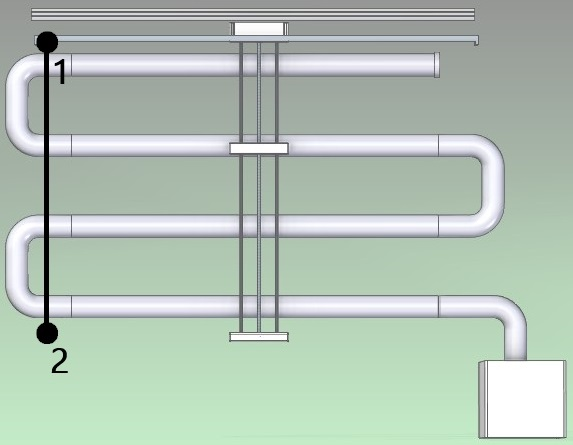
\includegraphics[width=0.6\textwidth]{imagenes/mov_vertical.jpg}
            \caption{\textit{Ruta escaneo vertical.}}
            \label{fig:estructura1}
    \end{figure}

    \item \underline{Escaneo horizontal por tubo}: Para cada tubo identificado, el robot se posiciona en su coordenada \textbf{Y} y ejecuta un barrido horizontal desde \textbf{X=0} hasta el límite derecho del workspace. Durante el movimiento continuo se detectan las cintas verticales que marcan las posiciones de las plantas.
    Al finalizar cada escaneo horizontal, el robot se mueve en diagonal hacia la posición \textbf{Y} del siguiente tubo, retornando a \textbf{X=0}. Este patrón se repite para todos los tubos. El escaneo horizontal siempre se ejecuta en la misma dirección (de izquierda a derecha).\\
        \begin{figure}[H]
        \centering
            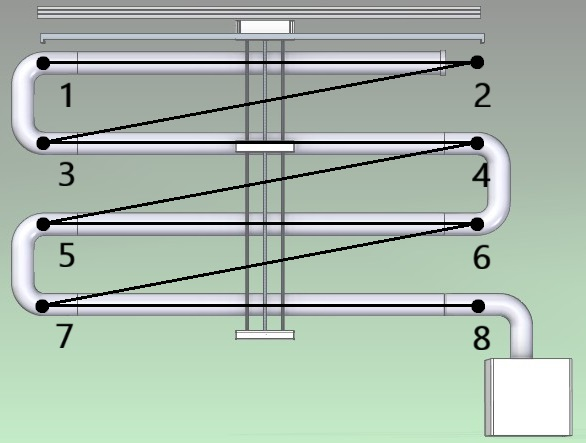
\includegraphics[width=0.6\textwidth]{imagenes/mov_total.jpg}
            \caption{\textit{Ruta escaneo horizontal.}}
            \label{fig:estructura2}
    \end{figure}

\end{enumerate}

Estructura del mapa.\\
\noindent
Los resultados se almacenan en una estructura de datos que contiene las coordenadas (X, Y) de cada posición de cultivo detectada. Durante la fase de cosecha, el sistema consulta este mapa para planificar la secuencia de visitas a las estaciones que contienen lechugas maduras.

El mapa se almacena periódicamente en formato JSON para permitir recuperación ante fallos y análisis posterior.
